\documentclass{article}


% if you need to pass options to natbib, use, e.g.:
%     \PassOptionsToPackage{numbers, compress}{natbib}
% before loading neurips_2024

\PassOptionsToPackage{numbers, compress}{natbib}

% ready for submission
\usepackage{neurips_2024}
\bibliographystyle{abbrvnat}

\usepackage[pdftex]{graphicx}

% to compile a preprint version, e.g., for submission to arXiv, add add the
% [preprint] option:
%     \usepackage[preprint]{neurips_2024}


% to compile a camera-ready version, add the [final] option, e.g.:
%     \usepackage[final]{neurips_2024}




\usepackage[utf8]{inputenc} % allow utf-8 input
\usepackage[T1]{fontenc}    % use 8-bit T1 fonts
\usepackage{hyperref}       % hyperlinks
\usepackage{url}            % simple URL typesetting
\usepackage{booktabs}       % professional-quality tables
\usepackage{amsfonts}       % blackboard math symbols
\usepackage{nicefrac}       % compact symbols for 1/2, etc.
\usepackage{microtype}      % microtypography
\usepackage{xcolor}         % colors


\title{Formatting Instructions For NeurIPS 2024}


% The \author macro works with any number of authors. There are two commands
% used to separate the names and addresses of multiple authors: \And and \AND.
%
% Using \And between authors leaves it to LaTeX to determine where to break the
% lines. Using \AND forces a line break at that point. So, if LaTeX puts 3 of 4
% authors names on the first line, and the last on the second line, try using
% \AND instead of \And before the third author name.


\author{%
  Rey Koki  \thanks{Use footnote for providing further information
    about author (webpage, alternative address)---\emph{not} for acknowledging
    funding agencies.} \\
  Department of Computer Science\\
  University of Colorado, Boulder\\
  Boulder, CO 80305\\
  \texttt{rey.koki@colorado.edu} \\
  % examples of more authors
  % \And
  % Coauthor \\
  % Affiliation \\
  % Address \\
  % \texttt{email} \\
  % \AND
  % Coauthor \\
  % Affiliation \\
  % Address \\
  % \texttt{email} \\
  % \And
  % Coauthor \\
  % Affiliation \\
  % Address \\
  % \texttt{email} \\
  % \And
  % Coauthor \\
  % Affiliation \\
  % Address \\
  % \texttt{email} \\
}


\begin{document}


\maketitle


\begin{abstract}
The increase in the frequency of wildfires on a global scale underscores the need for advancements in fire monitoring techniques for disaster management, environmental protection and to mitigate negative health outcomes. This research introduces an innovative, data-driven framework that leverages the semi-supervised method, pseudo-labeling, to generate smoke plume annotations in geostationary satellite imagery. The primary objective is to refine an existing National Oceanic and Atmospheric Administration smoke dataset that provides temporal and geographical information on individual smoke plumes but at variable and, primarily, low temporal resolution. To do this, we use deep learning and pseudo-labels to pinpoint the singular, most representative, satellite image that optimally illustrates the smoke annotation within the given time window. By identifying the most representative imagery of smoke plumes for a given smoke annotation, the study seeks to create an accurate and relevant machine learning dataset. The resulting dataset is anticipated to be an instrumental tool in developing further machine learning models, such as an automated system capable of real-time monitoring and annotation of smoke plumes directly from streaming satellite imagery.
\end{abstract}


\section{Introduction}

In recent years, the escalation of wildfire incidents worldwide has become a prominent environmental and public health concern. The combustion process in wildfires releases smoke containing fine particulate matter (PM2.5) and harmful gases, posing severe hazards to human health and air quality. These risks underscore the necessity for efficient and effective monitoring methods to mitigate the adverse health impacts associated with wildfire smoke. 

Traditionally, wildfire monitoring has relied on ground-based methods, such as forest service patrols, manned lookout towers, and aviation surveillance. While these methods provide valuable local insights, they are constrained by geographical and logistical limitations, often failing to deliver timely and comprehensive data, especially over large and remote areas. In contrast, satellite imagery offers a vantage point that overcomes these limitations, providing continuous, wide-area coverage and real-time data crucial for assessing and responding to the health risks posed by wildfire smoke.

Satellite imagery, equipped with advanced sensors, such as the Advanced Baseline Imager on the Geostationary Operational Environmental Satellites (GOES), have revolutionized environmental monitoring. These tools enable the detailed observation of smoke plumes, their particulate density, and the extent of smoke spread. These satellite-based systems offer the capabilities to provide critical insights into the concentration and movement of smoke particulates, facilitating accurate and timely assessments of air quality.

The integration of satellite imagery in wildfire smoke monitoring is not only instrumental in providing real-time data but also plays a significant role in public health planning and response. By mapping the spread and density of smoke, health authorities can issue timely warnings, implement evacuation protocols, and deploy resources effectively to mitigate health risks. Furthermore, long-term data gathered from satellite observations can aid in understanding the broader impacts of wildfire smoke on public health, influencing policy decisions and preventive measures.

Currently, multi-channel thresholding is a popular method to distinguish smoke pixels from pixels containing dust, clouds or other phenomenon with similar signatures. The method uses historical, labeled data to extract optimal radiance values for each channel that corresponds with the labeled class. These methods are tuned to particular biogeographies and often have issues with generalization to new locations with varying fuel types \cite{thresh_geog}.

In contrast to the numerical thresholding approach, human visual inspection of satellite imagery is another commonly used method for smoke identification. Trained analyst will inspect imagery and label the smoke by hand. This method is not as scalable as an automated approach and is limited by the availability of analysts and their time.

To address these challenges we can look towards innovative approaches and technological advancements in computer vision. Machine learning methods have shown potential in improving the accuracy and efficiency of satellite-based wildfire smoke detection and monitoring. For instance, SmokeNet, uses a convolutional neural network (CNN) based framework to determine if a scene of MODIS imagery contains smoke \cite{smokenet}. Another study also used a CNN to identify smoke on a pixel-wise basis using imagery from Himiwari-8 \cite{larsen}. Additionally, Wen et al. developed a CNN architecture that takes GOES-EAST imagery as input and National Oceanic and Atmospheric Administration (NOAA) generated annotations for the target labels during training \cite{smoke_goes}. 

The success of deep learning methods, such as CNNs, relies heavily on the availability of a large, representative dataset \cite{data_size}. Existing methods use relatively small amounts of data, from 57 \cite{wang} to 6825 \cite{smoke_goes}. In contrast, benchmark datasets for image classification contain tens of thosands (CIFAR-10 and MNIST) to millions (CIFAR-100 and ImageNet) of data samples. Keeping in mind the correlation between both the quality and quantity of data with model performance, we introduce the largest known smoke dataset, SmokeViz, containing over 100,000 independent samples.

\begin{table}[h]
    \caption{Comparison of different studies including method used, dataset size, satellite source, number of channels used and if the detection is done at a pixel or image level.}\label{studies}
    \centering
    \begin{tabular}{ccccrrcrc}
        \toprule
        Reference & Method & \verb|#| of Images & Satellite & \verb|#| Channels & Level\\
        \midrule
        \citep{smokenet}& CNN & 6255 & MODIS & 5 & image\\
        \citep{smoke_goes}& CNN & 6825 & GOES-EAST & 5 & pixel\\
        \citep{larsen} & CNN & 975 & Himiwari-8 & 7 & pixel\\
        \citep{wang}& U-Net & 47 & Landsat-8 & 13 & pixel\\
        SmokeViz  & U-Net & 100,000 & GOES-EAST/WEST & 3 & pixel\\
        \bottomrule
    \end{tabular}
\end{table}


A commonly used approach for increasing dataset size, semi-supervised learning leverages a labeled dataset to generate labels for an, often larger but unlabeled dataset. Pseudo-labeling, a form of semi-supervised learning, uses labeled data to train an initial model, then runs that model on unlabeled data to predict pseudo-labels, and finally trains a new model using the pseudo-labels \cite{pseudo}. We introduce a variation of pseudo-labeling not to increase the size, but to increase the quality of our dataset by using the pseudo-labels to choose the best satellite image out of a given time-window to represent each smoke plume annotation.


\section{Methods}
\subsection*{Dataset}

The initial data source, discussed in further detail in the next section, is uniquely characterized by each annotation having corresponding imagery ranging between 1-60 frames, where each frame captures 5 minutes of exposure.  Additionally, we have two satellite sensors, GOES-EAST and GOES-WEST, doubling the number of frames for a single annotation. We apply pseudo-labeling to develop a dataset that has a one-to-one annotation-to-image ratio, where we choose the best satellite image that represents where the smoke is located in the analyst annotation.

Dataset development came in three stages. First, we use the physics of light scattering to determine which singular satellite image would be in the optimal configuration for smoke detection. Second, we used that dataset to train an initial model that will identify smoke in satellite imagery. Third, we use that initial model to label each satellite image in a given annotation's time-window and the optimal satellite image is chosen based on which image's pseudo-labels has the greatest overlap with the analyst annotation for the given location and densities of smoke.

\subsubsection*{Smoke Labels} 
The National Environmental Satellite, Data and Information Service (NESDIS) and NOAA manage environmental satellite programs such as the Hazard Mapping System (HMS) \citep{hms, hms_val}. The HMS program is an operational system that uses an aggregation of satellite data to generate active fire and smoke data that is used in applications such as air quality assessments and serves as verification and validation for NOAA's smoke forecasting model, HYSPLiT, \citep{hysplit_ver}. To train our model, we implement a supervised learning framework that uses the HMS analyst smoke product as truth labels during the model training process.

HMS smoke analysis data gives the coordinates of the smoke perimeter and classifies the smoke by density within a given time window. The time windows can range from instantaneous (same start/end time) to lengths of 5 hours. While the bounds of the smoke annotations can change within the larger time spans, the analyst is making an approximation that should reflect the smoke coverage over the duration of the window. The density information is qualitatively determined by the analyst based on smoke opacity and categorized as either light, medium or heavy as seen in figure \ref{densities}a.

\begin{figure}
    \centering
    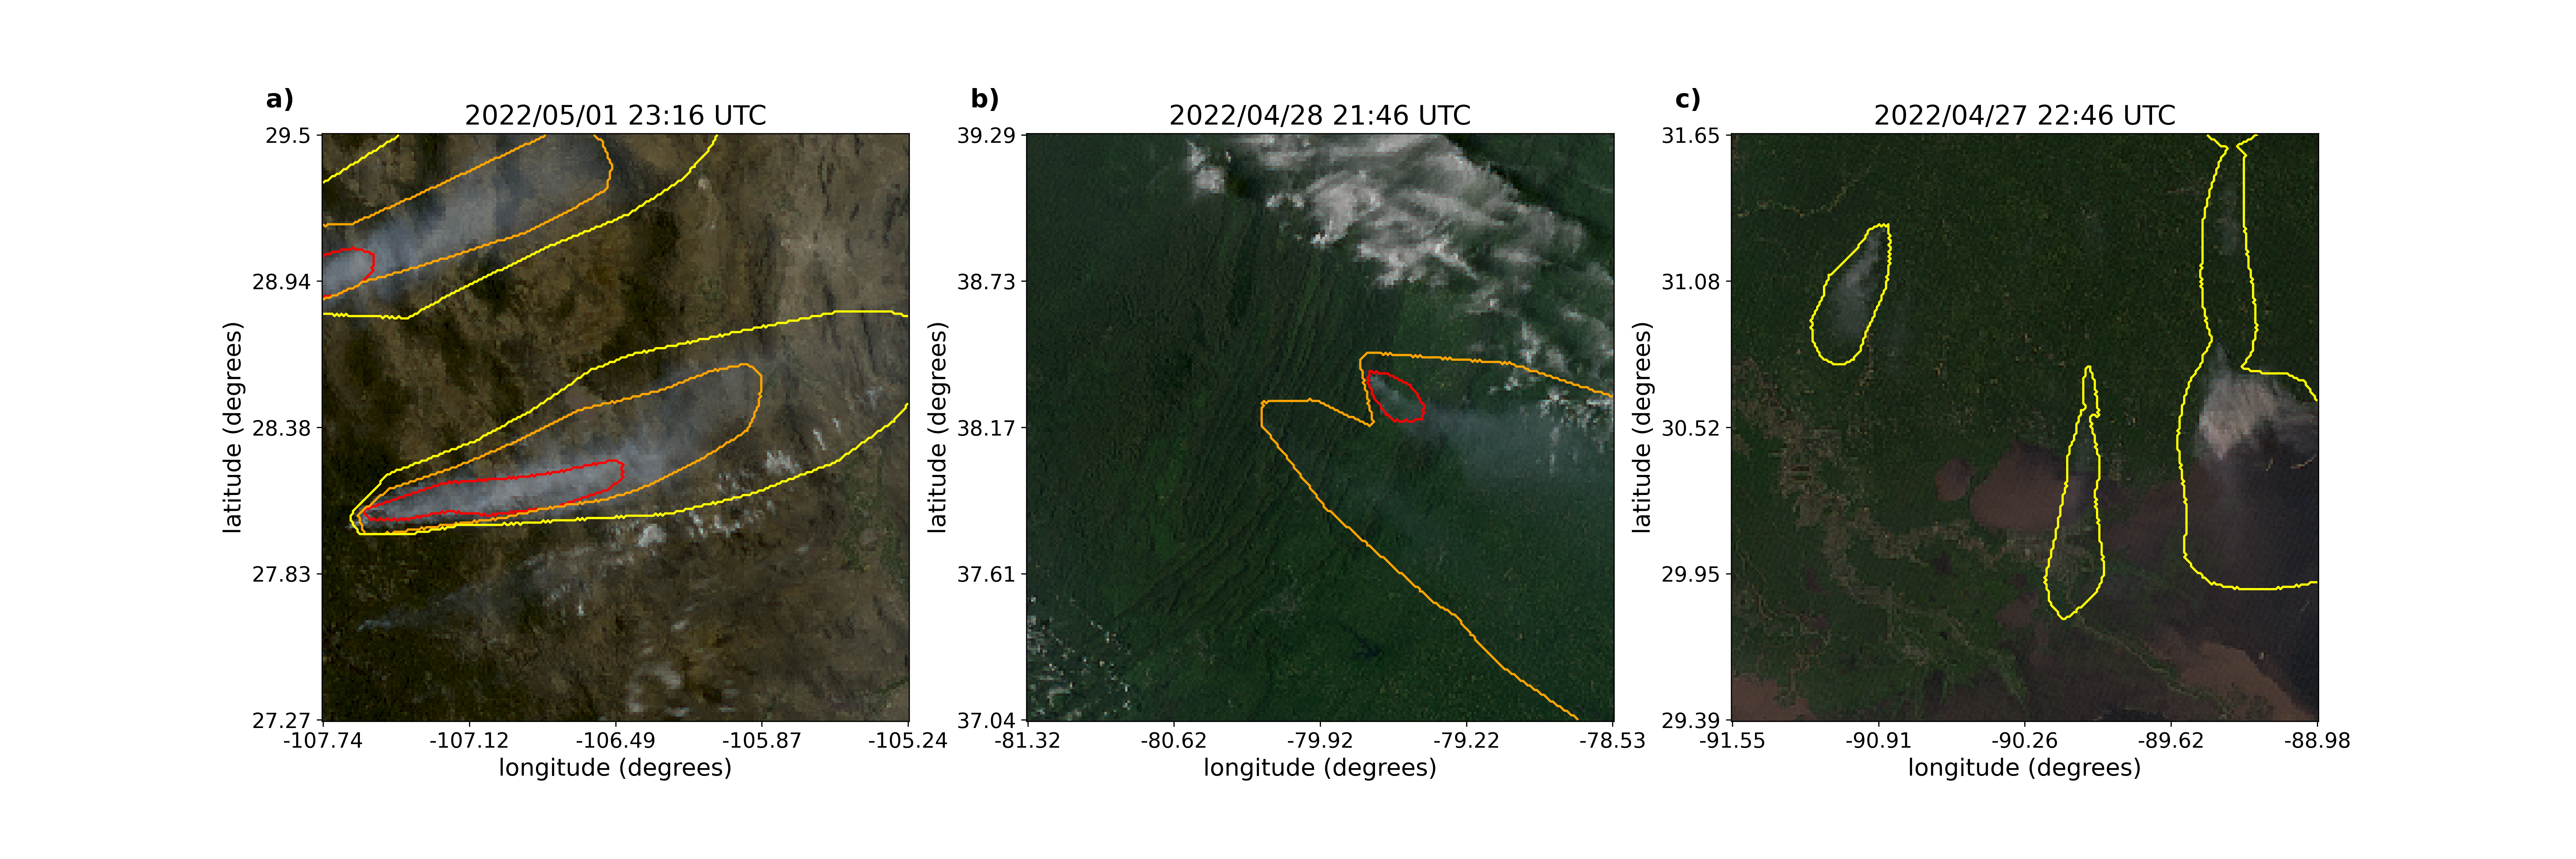
\includegraphics[width=15cm]{figures/Misclassified.png}
    \caption{Satellite imagery captured by GOES-EAST within a few days of each other. The yellow, orange and red contours indicate the extent of Light, Medium and Heavy smoke.  a) shows a canonical example of a smoke plume. b) and c) show variations in the density labels. b) we show Medium and Heavy densities of smoke that, upon visual inspection, could be interpreted as less dense than portions of the Light density smoke labeled in c).}\label{densities}
\end{figure}

\subsubsection*{Thermometer Encoding Smoke Densities}

One of the challenges introduced with using human generated qualitative smoke densities was that, as seen in figure \ref{densities}b and \ref{densities}c, there are variations in what is labeled as heavy or light density smoke. More generally, reproducing qualitative metrics with quantitative algorithms is a challenging problem, but we apply mathematical approaches that mitigate some of the underlying complications of our specific problem. Despite the fact that the smoke densities introduce qualitative complexities, we decided that the density approximations were important to use in our dataset because of the differences in signatures the densities produce. Within the satellite imagery, the appearance of a light density smoke plume will look significantly different than a heavy density smoke plume as seen in figure \ref{densities}. Additionally, a light density smoke plume is expected to be more challenging to detect since it is easier for it to be misclassified as not smoke. During the training process, the separate density categories allows us to deferentially weight the penalization given to the model for incorrect classifications based on category. For example, the model can be given a small penalization for misclassifying light smoke as not smoke while given a higher penalization for misclassifying heavy smoke as not smoke. 

In addition to the densities being ordered and categorical, the differences between the density categories are not evenly distributed by a metric, such as particulate matter per square meter. The intervals between densities being unknown along with the hierarchical nature of the density labels makes the labels ordinal instead of just categorical. This data property allows us to use thermometer encoding, which leverages the idea that heavy density smoke includes both medium and light density smoke, that heavy density smoke is closer to medium than it is to light and automatically weights the loss functions and incorporates the ranked ordering of the densities.  As seen in Table \ref{therm}, one-hot encoding, commonly used for categorical data, doesn't take ordinal properties of the data into consideration.  

\begin{table}[h] 
    \caption{A comparison of one-hot encoding used for categorical data to thermometer encoding for ordinal data.}\label{therm}
    \centering
    \begin{tabular}{ccccrrcrc}
        \toprule
        category & one-hot & thermometer \\
        \midrule
        No Smoke & \texttt{[0 0 0]} & \texttt{[0 0 0]} \\
        Light  & \texttt{[0 0 1]} & \texttt{[0 0 1]} \\
        Medium & \texttt{[0 1 0]} & \texttt{[0 1 1]} \\
        Heavy  & \texttt{[1 0 0]} & \texttt{[1 1 1]} \\
        \bottomrule
    \end{tabular}
\end{table}

\subsubsection*{Time Windows For Smoke Annotations}

In order to take into account movement characteristics to help identify smoke, analysts use multi-frame animations of the satellite imagery. The resulting annotations often have large time windows over multiple hours to represent one smoke plume. Since their goal is to show the general coverage over that time span, often the smoke boundaries don't match up with the satellite imagery over the entire time window \ref{timelapse}. One way to approach this problem would be to use all the satellite images the analysts used as input. Since the timespans are non-uniform, this would vary the length in imagery inputs into the model, which would be difficult with a CNN architecture. Moreover, this would require a large amount of additional memory and computational resources. Instead of using the original analysts' many satellite image inputs to one annotated output, we develop a one-to-one input-to-output by finding the optimal singular satellite image input to represent the annotation. As
discussed in the next section, we do this by making physics-driven choices on which satellite and timestamp would give the optimal angle between the sun and satellite that would produce the strongest smoke signature for the geolocation and timestamp of the smoke plume. 


\begin{figure} \label{timelapse}
    \centering
    \includegraphics[width=16cm]{figures/timelapse.png}
    \caption{True Color GOES imagery from May 2022, Southeast New Mexico (\(31^{\circ}\)N, \(100^{\circ}\)W) during the start of the Foster Fire. The HMS annotations for the smoke outlines shown here spanned from 19:10\textendash23:00 UTC but visually match the smoke location for the last part of the timewindow.}
\end{figure}


\subsubsection*{Satellite Imagery} 

The Geostationary Operational Environmental Satellites (GOES) are operated by the NOAA and NESDIS support meteorology research and forecasting for the United States. We use the latest operational satellites, GOES-16 (EAST), 17 and 18 (WEST) that carry the Advanced Baseline Imager (ABI), that measure 16 bands between the visible and infrared wavelengths. In improvement to the GOES predecessors, imagery is collected every 5 minutes for the contiguous United States and every 10 minutes for the full disk. We use bands 1-3 (Table \ref{rgb_bands}) as input to Satpy's composite algorithm to develop a true color image representation, similar to what is used as input by HMS analysts \citep{satpy} and \citep{true_color}.

\begin{table}
    \caption{To create a true color image, we use the following bands from the Advanced Baseline Imager Level 1b CONUS (ABI-L1b-RadC) product.}\label{rgb_bands}
    \centering
        \begin{tabular}{ccccrrcrc}
            \toprule
            band & description & center wavelength & spatial resolution (km)\\
            \midrule
            C01 &  blue visible & 0.47 & 1 \\
            C02 & red visible & 0.64 & 0.5 \\
            C03 & veggie near infrared & 0.865 & 1 \\
            \bottomrule
        \end{tabular}
\end{table}

We used a physics-informed approach in selecting the initial dataset for training our model. Rather than use the cumulative data from GOES-WEST and GOES-EAST images, we select one or the other based on the solar zenith angle. For smoke identification, this approach can achieve a much higher signal-to-noise than imaging the earth’s surface from an arbitrary angle. The elastic scattering of light is the primary mechanism to account for - while the atmosphere is composed of molecules with size 


[<1]nm, smoke particles can vary from 100 nm - 10 \(\mu\)m in diameter, \(d\). The GOES ABI covers spectral bands from 0.47 \(\mu\)m - 13.3 \(\mu\)m, so atmospheric and smoke particle sizes occupy two very different regimes with respect to the imaging wavelength \(\lambda\), as shown in figure \ref{regime}. In the extreme limit of \(\lambda \gg d\), the physics of scattering of light off a small sphere is captured by Rayleigh scattering. This process has two critical consequences: (1) the scattering cross section of light is strongly wavelength dependent (scaling with \(\lambda^{-4}\)), meaning that photons with wavelength closer to the ultraviolet are scattered more strongly than infrared photons. (2) the scattering cross section scales with an angular dependent cross section of \((1 + \cos^2 \theta)\). Scattered photons follow the emission distribution of a radiating dipole, scattering more strongly in the forward and backwards directions \((\theta = 0,\pi)\)than orthogonal to the direction of propagation \((\theta = \pi/2, 3\pi/2)\), see figure \ref{mei} for Rayleigh scattering schematic.

\begin{figure}
    \centering
    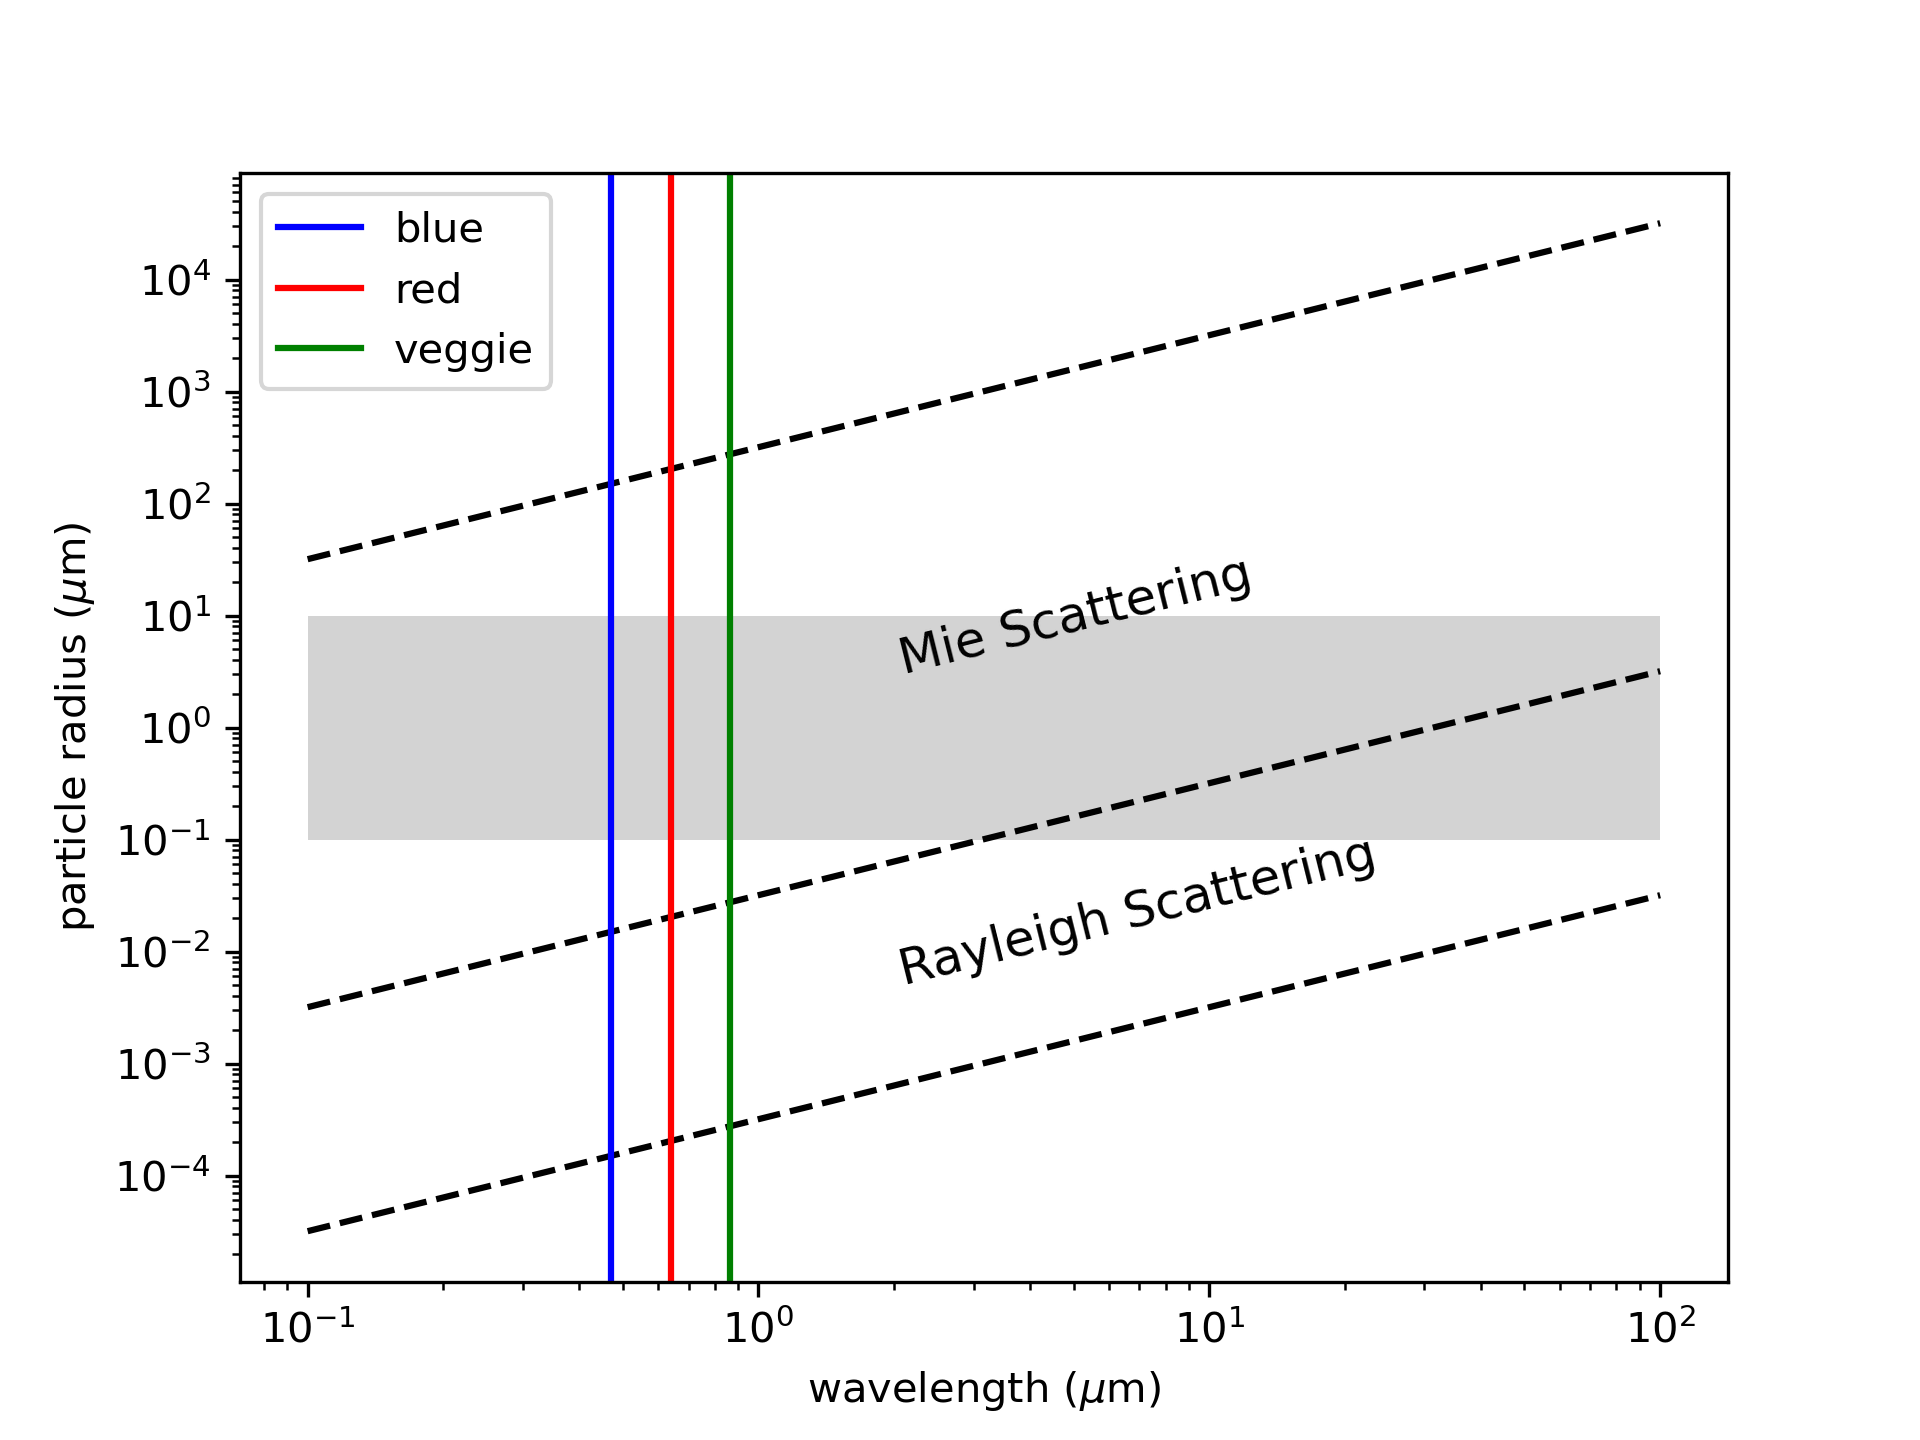
\includegraphics[width=10cm]{figures/scatter_regime.png}
    \caption{Relationship between the size of a particle, the wavelength of light interacting with the particle and the type of scattering behavior induced by that interaction. The dotted lines represent rough estimates of the boundaries between the scattering regimes \citep{petty}. The gray area represents the range of particle radius relevant to smoke particulate matter.}\label{regime}
\end{figure}

\begin{figure}
    \centering
    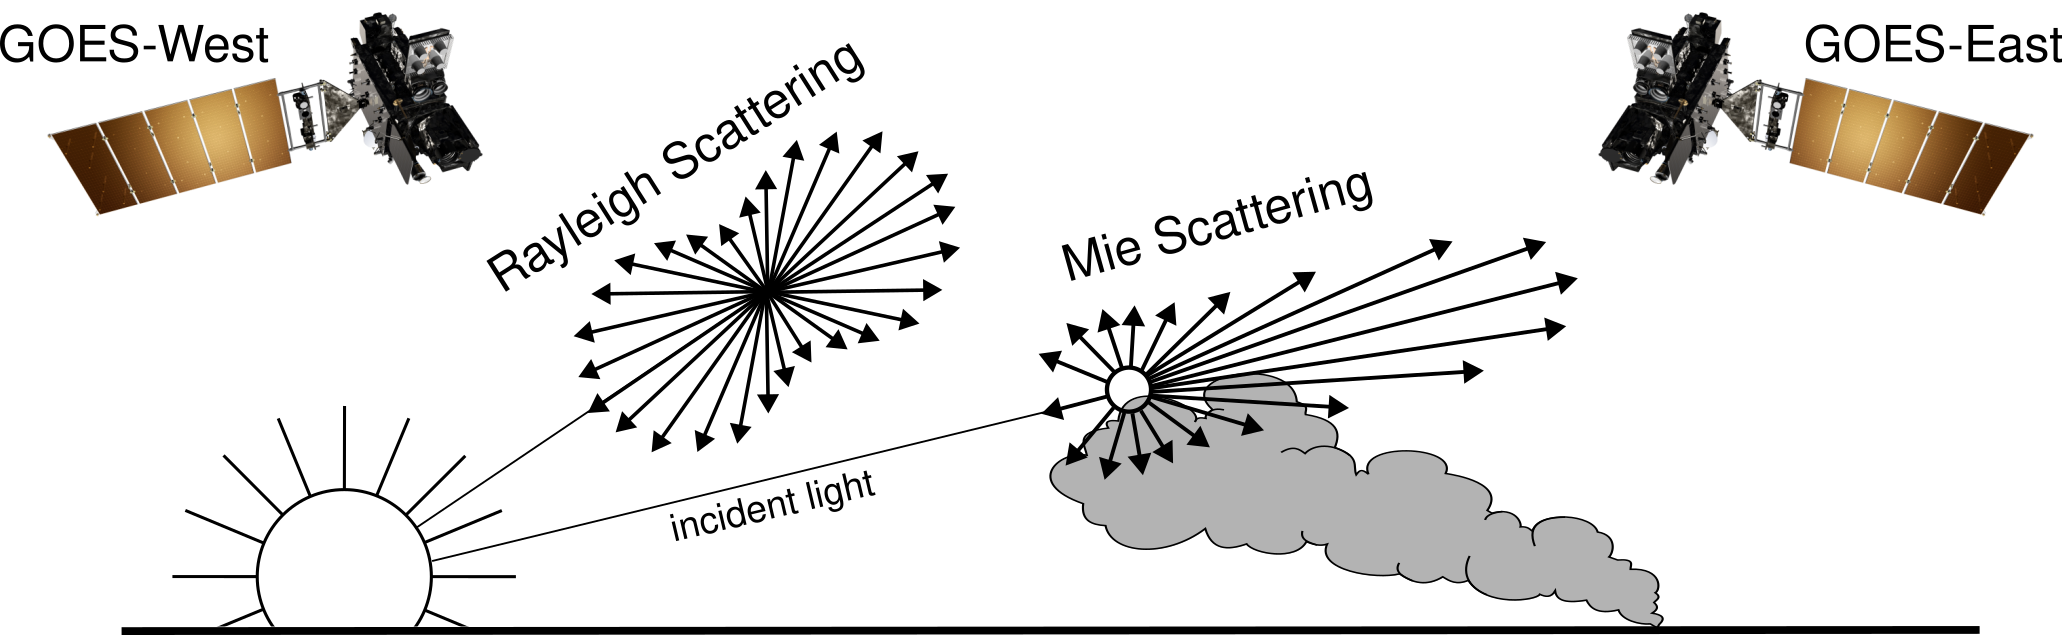
\includegraphics[width=10cm]{figures/mei.png}
    \caption{If the particle size is \(<\frac{1}{10}\) the wavelength of the interacting light, then the primary scattering will be Rayleigh. Mie scattering is the predominant scattering mechanism when the particle size is larger than wavelength of light.} \label{mei}
\end{figure}

The significance of these scalings is that the observer, or detector, will receive blue photons in most directions orthogonal to the source. Equivalently, photons traveling colinearly with line of sight to the emission source will mostly have wavelengths in the infrared band. 


In the converse regime of \(d > \lambda\)


, the elastic scattering of light against matter is modeled through Mie scattering. Unlike Rayleigh scattering, Mie scattering is largely wavelength independent and has a more complicated radiation pattern where the cross section has a maximal amplitude in the forward direction. An observer downstream of this scatterer will collect more photons than one positioned directly behind it. In the context of smoke identification, a sunrise or sunset will lead to a higher Mie scattered signal in GOES-WEST and GOES-EAST respectively, as shown with a smoke plume producing a stronger signal in GOES-EAST imagery near sunset in figure \ref{16_vs_17}.

\begin{figure}\label{16_vs_17}
    \centering
    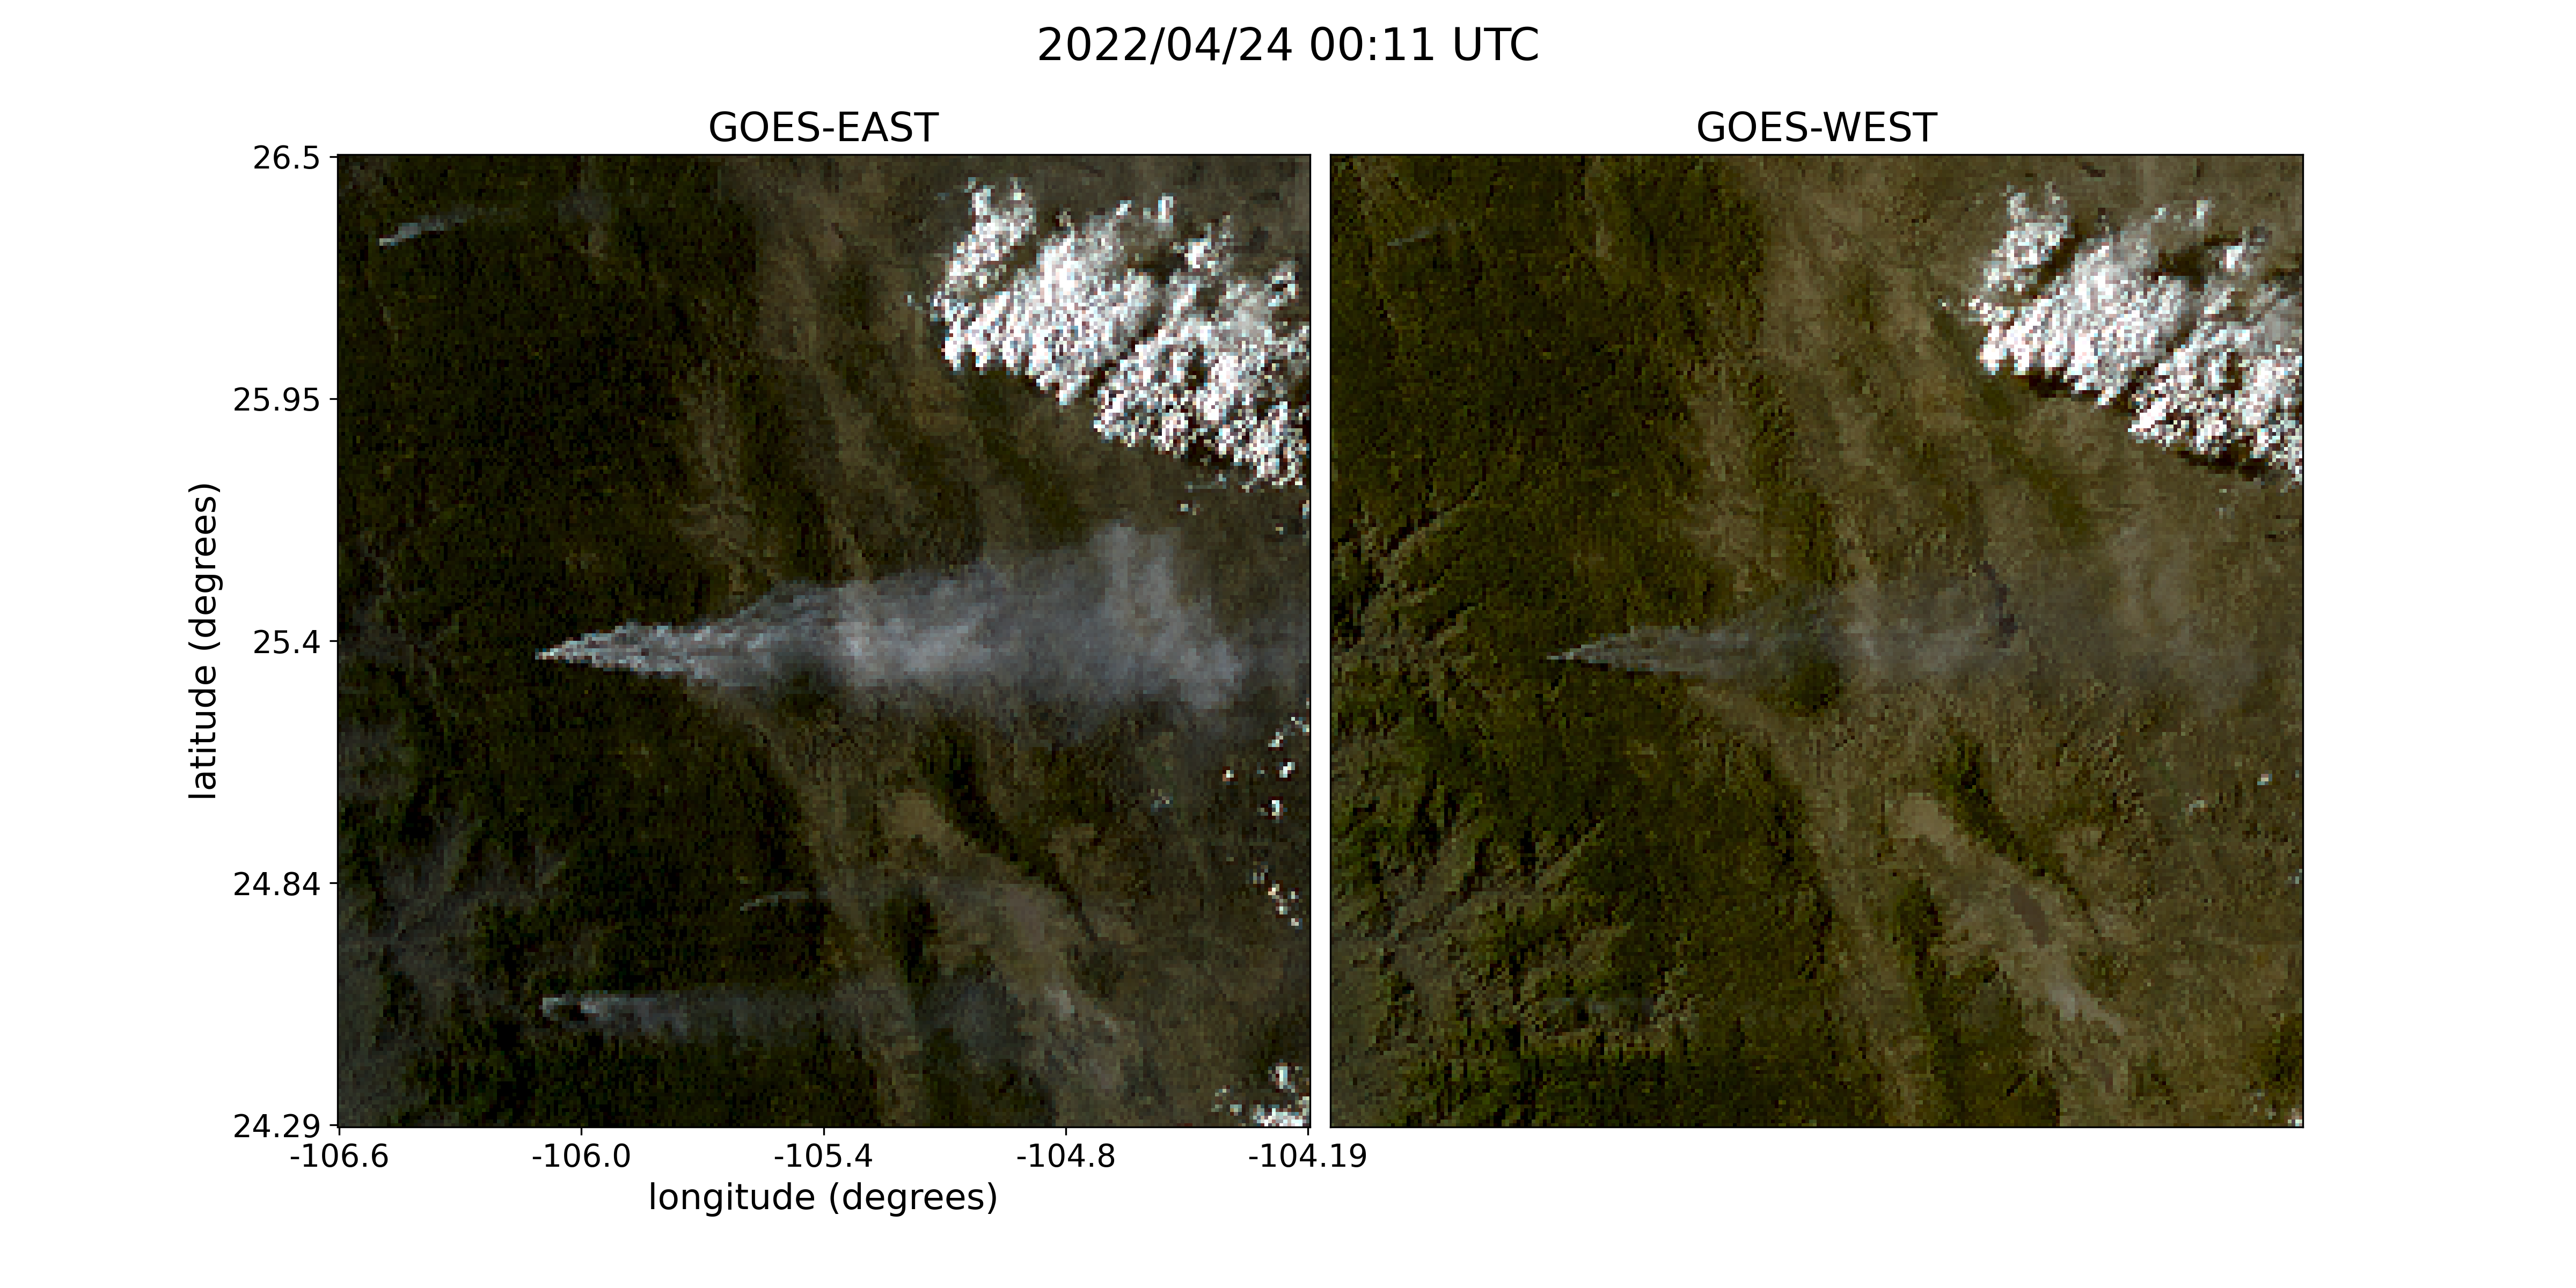
\includegraphics[width=15cm]{figures/G16_v_G17.png}
    \caption{True Color GOES-EAST (left) and GOES-WEST (right) imagery from April \(24^{th}\), 2022. The images were taken about 1.5 hours before sunset for this geolocation and time of year (01:43 UTC).}\label{16vs17}
\end{figure}

Smoke identification therefore amounts to extracting a signal of \(d > \lambda\) photons from the \(\lambda \gg d\) background. Positioning a detector along line of sight to the scatterer will result in a higher signal from smoke particles (figure \ref{mei}). Filtering the imaged wavelength can enhance this signal; photons collected in the blue spectrum will have a naturally lower background along the line of sight to the illumination source do their high level of Rayleigh scattering as. Therefore, as demonstrated in figure \ref{bands}, this configuration results in the highest signal to noise imaging for smoke particles. 



\begin{figure}
    \centering
    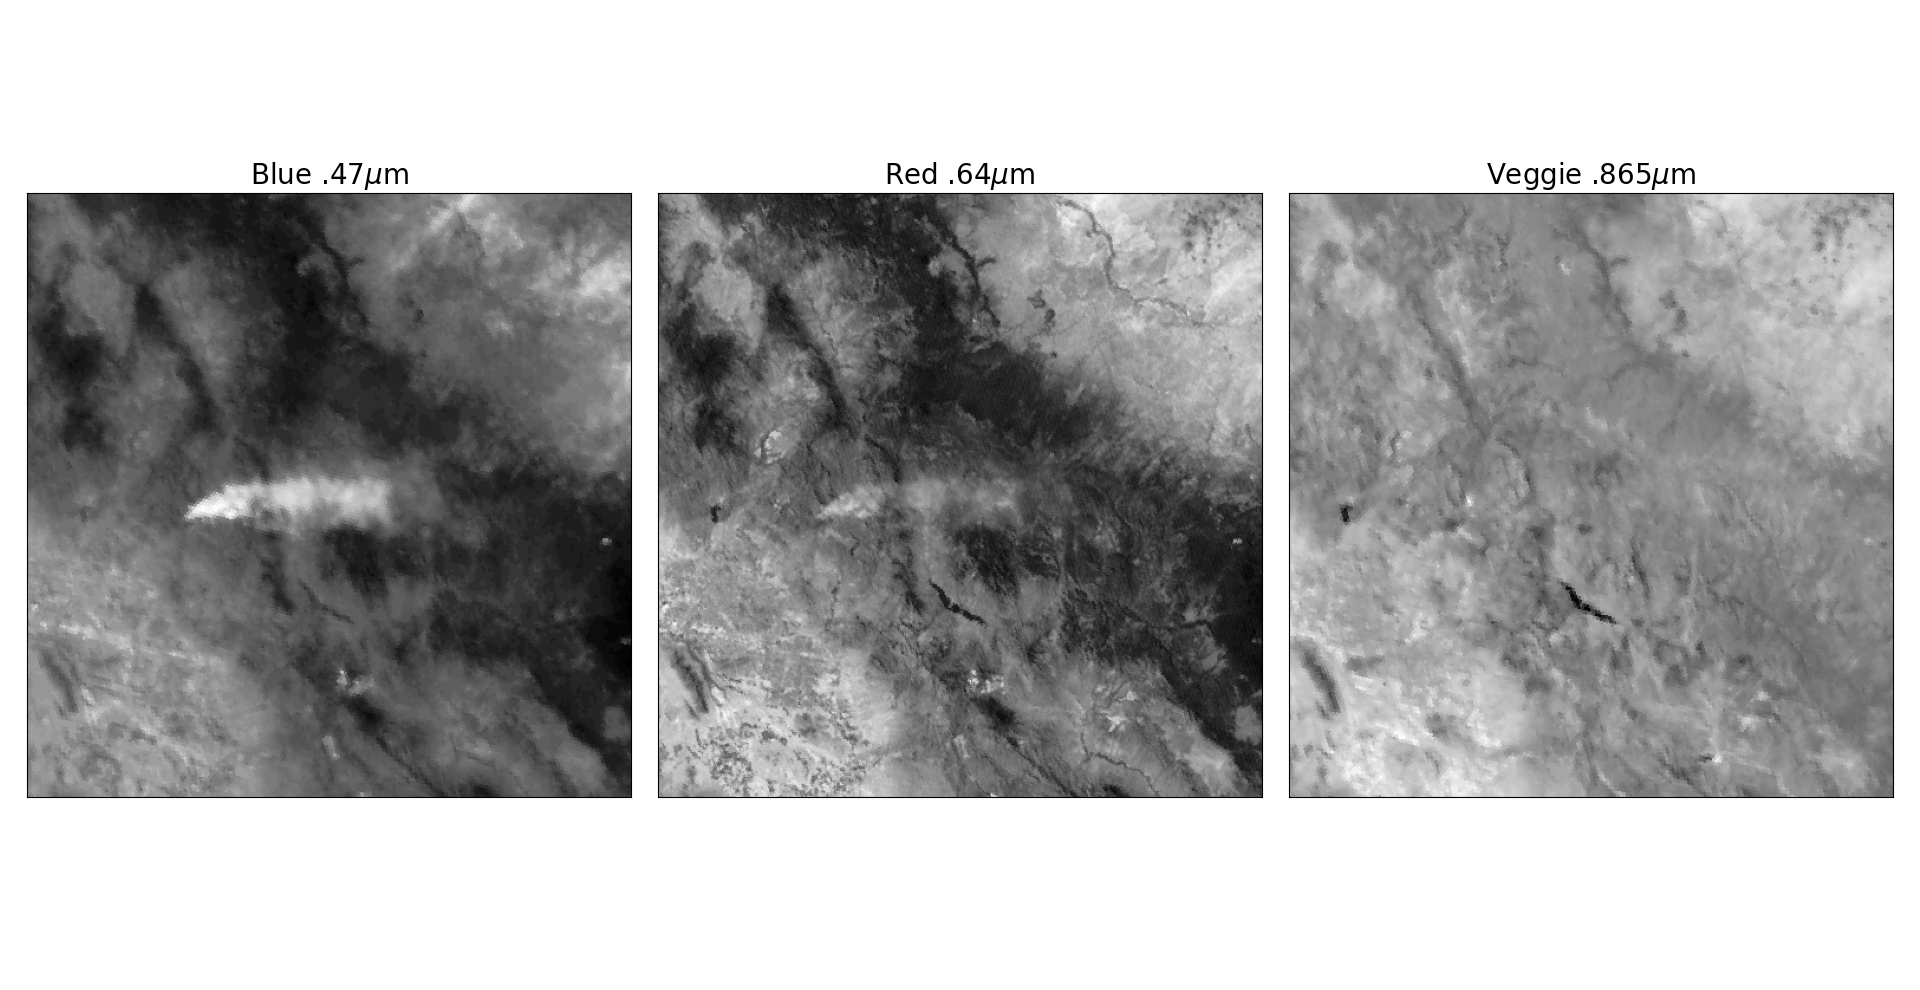
\includegraphics[width=16cm]{figures/GOES16_bands.png}
    \caption{The three bands of GOES-EAST data are the raw input to generate the True Color image shown in figure \ref{16vs17}. There appears to be a higher signal-to-noise ratio for smoke detection as the wavelength, \(\lambda\), of light being measured decreases.}\label{bands}
\end{figure}





Based on these criteria, the optimal strategy is to pull data from GOES-WEST right after sunrise and from GOES-EAST right before sunset. Another consideration to account for was that when the sun is in optimal alignment with the satellite for detecting smoke also coincides with the maximal amount of atmosphere the light travels through. This is shown in figure \ref{G17_sunrise}, where the noise introduced by higher amounts of atmospheric interactions can obfuscate the signal from the smoke, despite the smoke signal being at its highest. This phenomenon is even more prominent the further the smoke is longitudinally from the satellite since the light must travel through more atmosphere between scattering off the smoke and reaching the detector. Additionally shown in figure \ref{G17_sunrise}, and is especially evident for data close to sunrise, when the time window is large, the smoke has often not dispersed to the extent of the analysts' annotation boundaries. We consider the atmospheric interaction noise in our algorithms to develop the dataset by choosing a lag time between sunrise and optimal image timestamp as a function of longitude. 

The resulting algorithm used atmospheric properties and light scattering physics to make an estimate of which singular satellite image within the analyst time-window would give the best representation of the smoke plume label. That dataset was then used to train a model that would generate pseudo-labels for every image within the time-window and choose the image with the highest alignment between smoke in the image and annotation.


\begin{figure}
    \centering
    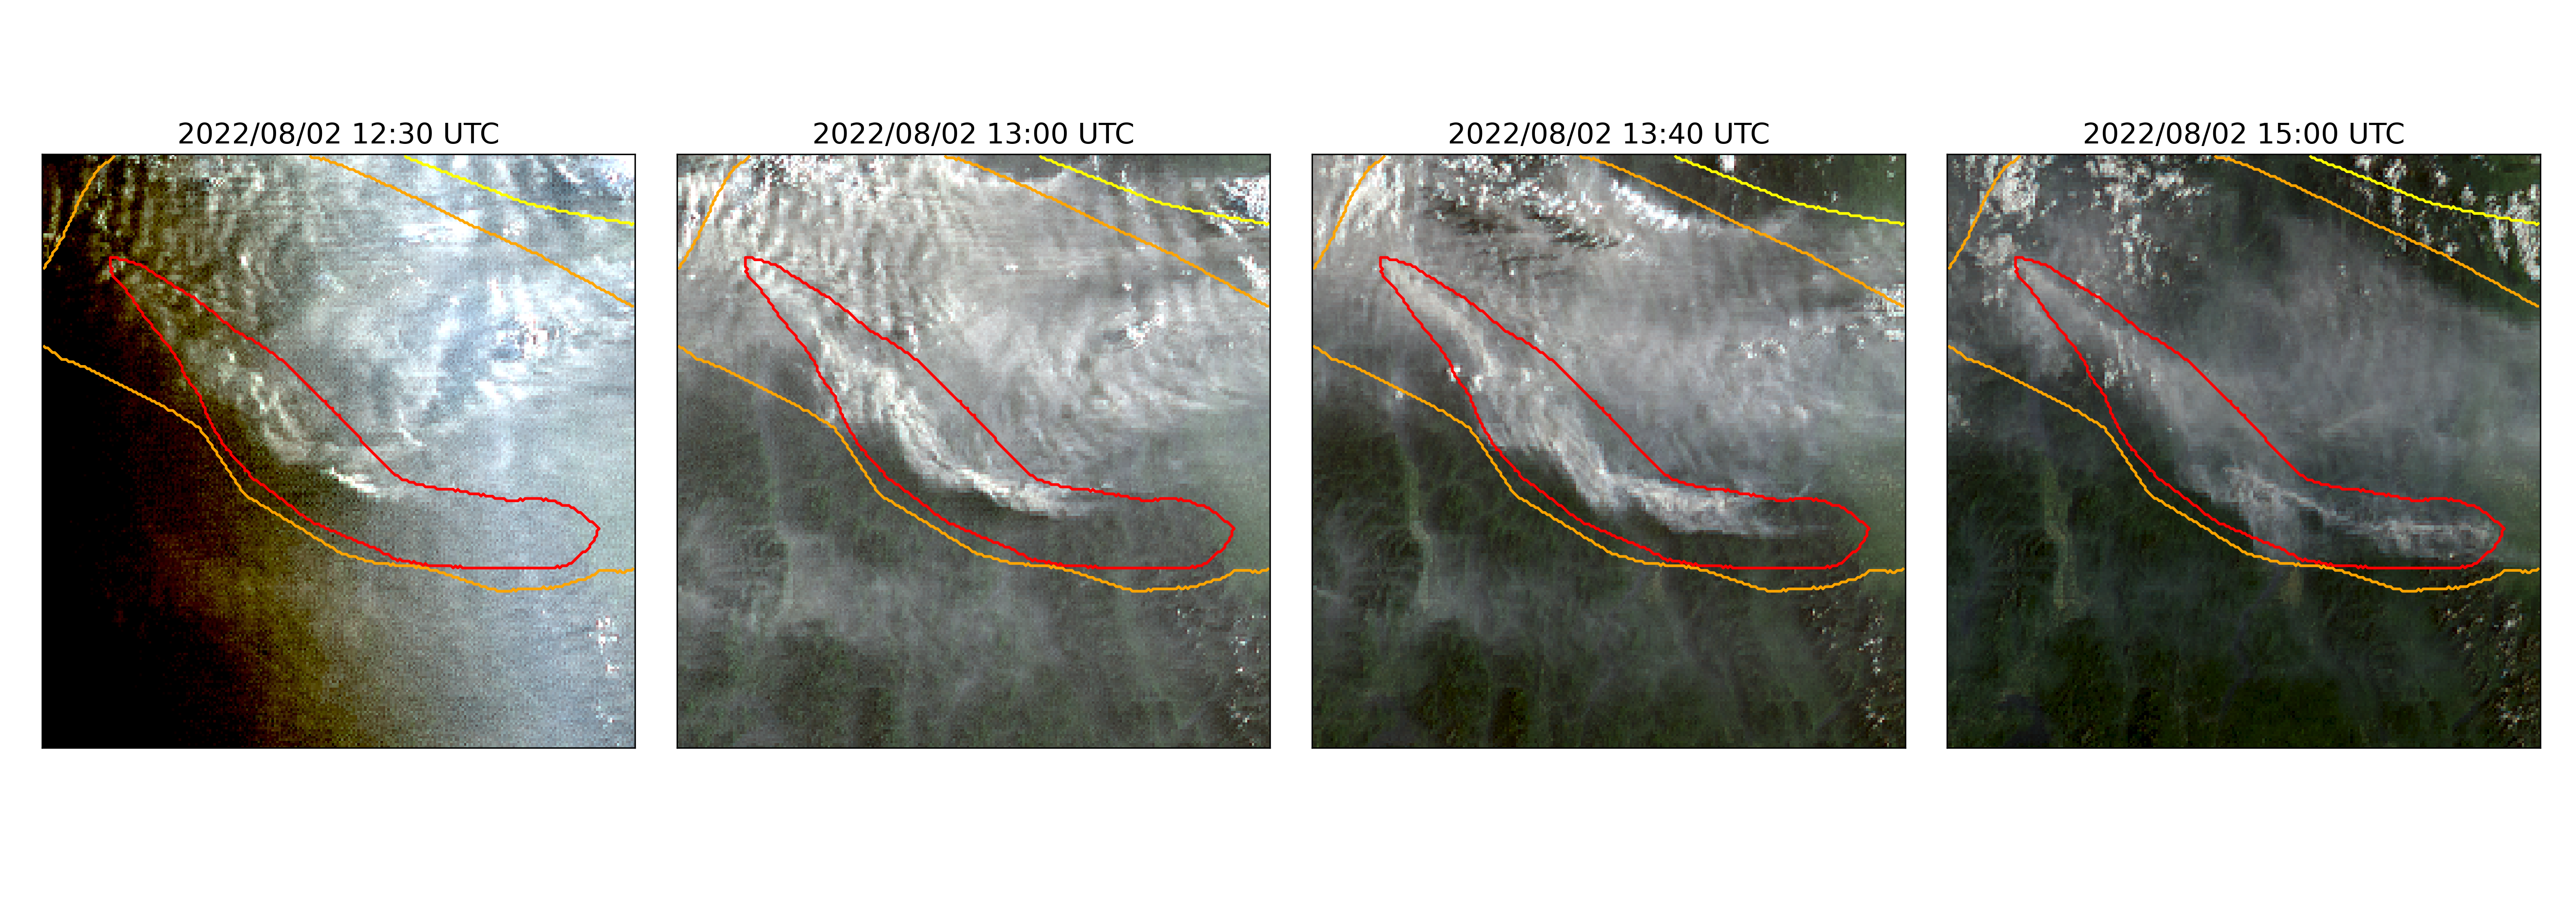
\includegraphics[width=16cm]{figures/timelapse_G17_2.png}
    \caption{A smoke annotation projected onto GOES-WEST imagery from August 2022 that spans from 11:00 UTC to 15:00 UTC, sunrise on August 2nd, 2022 at coordinates (49°24'N, 115°29'W) was 12:15 UTC. 15 minutes after the calculated sunrise, the imagery contains a noticeably higher levels of noise than the subsequent imagery that's light travels through (thus interacts with) less atmosphere as the sun rises and the angle between GOES-WEST and the sun decreases. }\label{G17_sunrise}
\end{figure}




\subsubsection*{Machine Learning Model} 

We implement a deep learning architecture that uses the encoder from the ResNet model \citep{resnet} and a semantic segmentation classifier from the U-Net model \citep{unet}. Transfer learning has shown to reduce the time and resources needed to train a model by leveraging information from pre-trained models \citep{transfer}, \citep{transfer2}.  We initialize the values of our model weights using the pre-trained values originally trained on the ImageNet dataset \citep{imgnet}, containing 1.2 million images and 1000 categories. Our model was developed using the Segmentation Models PyTorch package \citep{semantic} that was written as a high level API for implementing models for semantic segmentation problems.  We input 256x256x3 snapshots of True Color GOES imagery that contains smoke and output a 256x256x3 classification map that predicts if a pixel contains smoke and if so, what the density of that smoke is. As mentioned earlier, we apply the thermometer encoding shown in table \ref{therm} to encode the smoke densities and apply binary cross entropy as the loss function per density of smoke. 

The original dataset developed using the Mie algorithm contained over 120,000 samples. To train our model, we split the dataset into training (95,000 samples), validation (12,000 samples) and testing (12,000) datasets. Training data contains data from the years 2018, 2019, 2020, 2021 and 2023 while the data from 2022 is split into validation and testing data by taking data from alternating weeks of the year. Splitting 2022 data by week allowed us to leave more full years of data for the training set and allowed each dataset to show yearlong trends while trying to keep the datasets independent from one another.

We trained a model over 20 epochs and then used that model to develop the dataset by determining which satellite image provided the best Intersection over Union (IoU) value. The IoU metric is given by the ratio of area of overlap to the area of union as defined in equation \ref{iou}, where A and B are the truth labels and the model's predictions.

\begin{equation} \label{iou}
    IoU = \frac{| A \cap B|}{|A|\cup|B|}
\end{equation}

To determine which image best represents the analyst annotation, we gather all the satellite imagery for the given time window and run them through the machine learning model. The output of the model gives a prediction on if there is smoke in the image, and if there is smoke, where the smoke is in that image and what the density of that smoke is. The model output generates pseudo-labels for each density of smoke that are compared to the analyst annotations. To compare the pseudo labels and analyst labels, we calculate the IoU using the total set of pixels for the pseudo-labels at that density of smoke and the entire set of pixels for the analyst labels for a particular smoke density in each image. The image with the highest IoU score is chosen as the image that best represents the analyst smoke annotation. Generally, a confidence threshold value is defined to decide if a pseudo-label should to be included in a dataset \citep{conf_thresh}. We chose a confidence threshold that would include the sample in the dataset if the maximum IoU value was over 0.1.



\section*{Results}

To interpret the performance of our trained model, we report the IoU metrics in table \ref{iou_results} that were computed by running the model on the Mie algorithm derived dataset and the pseudo-labeled dataset. For each density, we calculate the IoU using the total set of pixels that the model predicts as that density of smoke and the entire set of pixels labeled by the analyst as a particular smoke density over all imagery contained in the testing dataset. Additionally, we compute the overall IoU for all densities by first computing the number of pixels that intersect their correct density and divide that by the total number of pixels that make up the union of model predicted and analyst labeled smoke as shown in equation \ref{overall_iou}.


\begin{equation} \label{overall_iou}
    IoU_{overall} = \frac{\sum\limits_{i=light}^{heavy}|A_{i}\cap B_{i}|  }{\sum\limits_{i=light}^{heavy}|A_{i}|\cup|B_{i}|}
\end{equation}

\begin{table} 
    \caption{IoU results per density of smoke and over all densities.}\label{iou_results}
    \centering
    \begin{tabular}{ccccrrcrc}
        \toprule
        category & IoU Mie Dataset & IoU Pseudo-Labeled Dataset \\ 
        \midrule
        Light  & 0.394 &  0.551 \\
        Medium & 0.283 &  0.392 \\
        Heavy  & 0.233 &  0.290 \\
        Overall & 0.365 &  0.510 \\
        \bottomrule
    \end{tabular}
\end{table}



\section{Conclusion}




In this study, we have refined an existing dataset originally curated by the HMS team, transforming it from a many-to-one imagery-to-annotation format to a, more concise, one-to-one satellite image-to-annotation dataset. The initial HMS dataset primarily gave an approximation of where smoke had been present for a given time window, though it did not confirm the actual existence of smoke in the pixels of the selected images. Due to that nature of the HMS dataset, our Mie derived dataset gave an approximation of when we'd best be able to measure the smoke signal but did not factor in if the smoke was actually present in the selected image. This discrepancy can be detrimental when training a machine learning model, as it may penalize accurate predictions and inadvertently introduce biases towards misclassifying noise as meaningful signal. 

To make improvements on the dataset's reliability, we apply a machine learning model trained on the Mie-derived dataset to select the satellite image within the time-frame that best overlaps with the analyst's annotation. A notable illustration of the improvements introduced by the machine learning method is evident in Figure \ref{ml_vs_mei}. The annotation associated with this example encompasses five hours of imagery and we show the images that is chosen by each of our two methods. While the Mie algorithm tries to optimize for the highest possible signal-to-noise, which is the image closest to sunrise, our machine learning algorithm chooses the image that maximizes the overlap of smoke predicted by the model with the analyst's annotation.



\begin{figure}
    \centering
    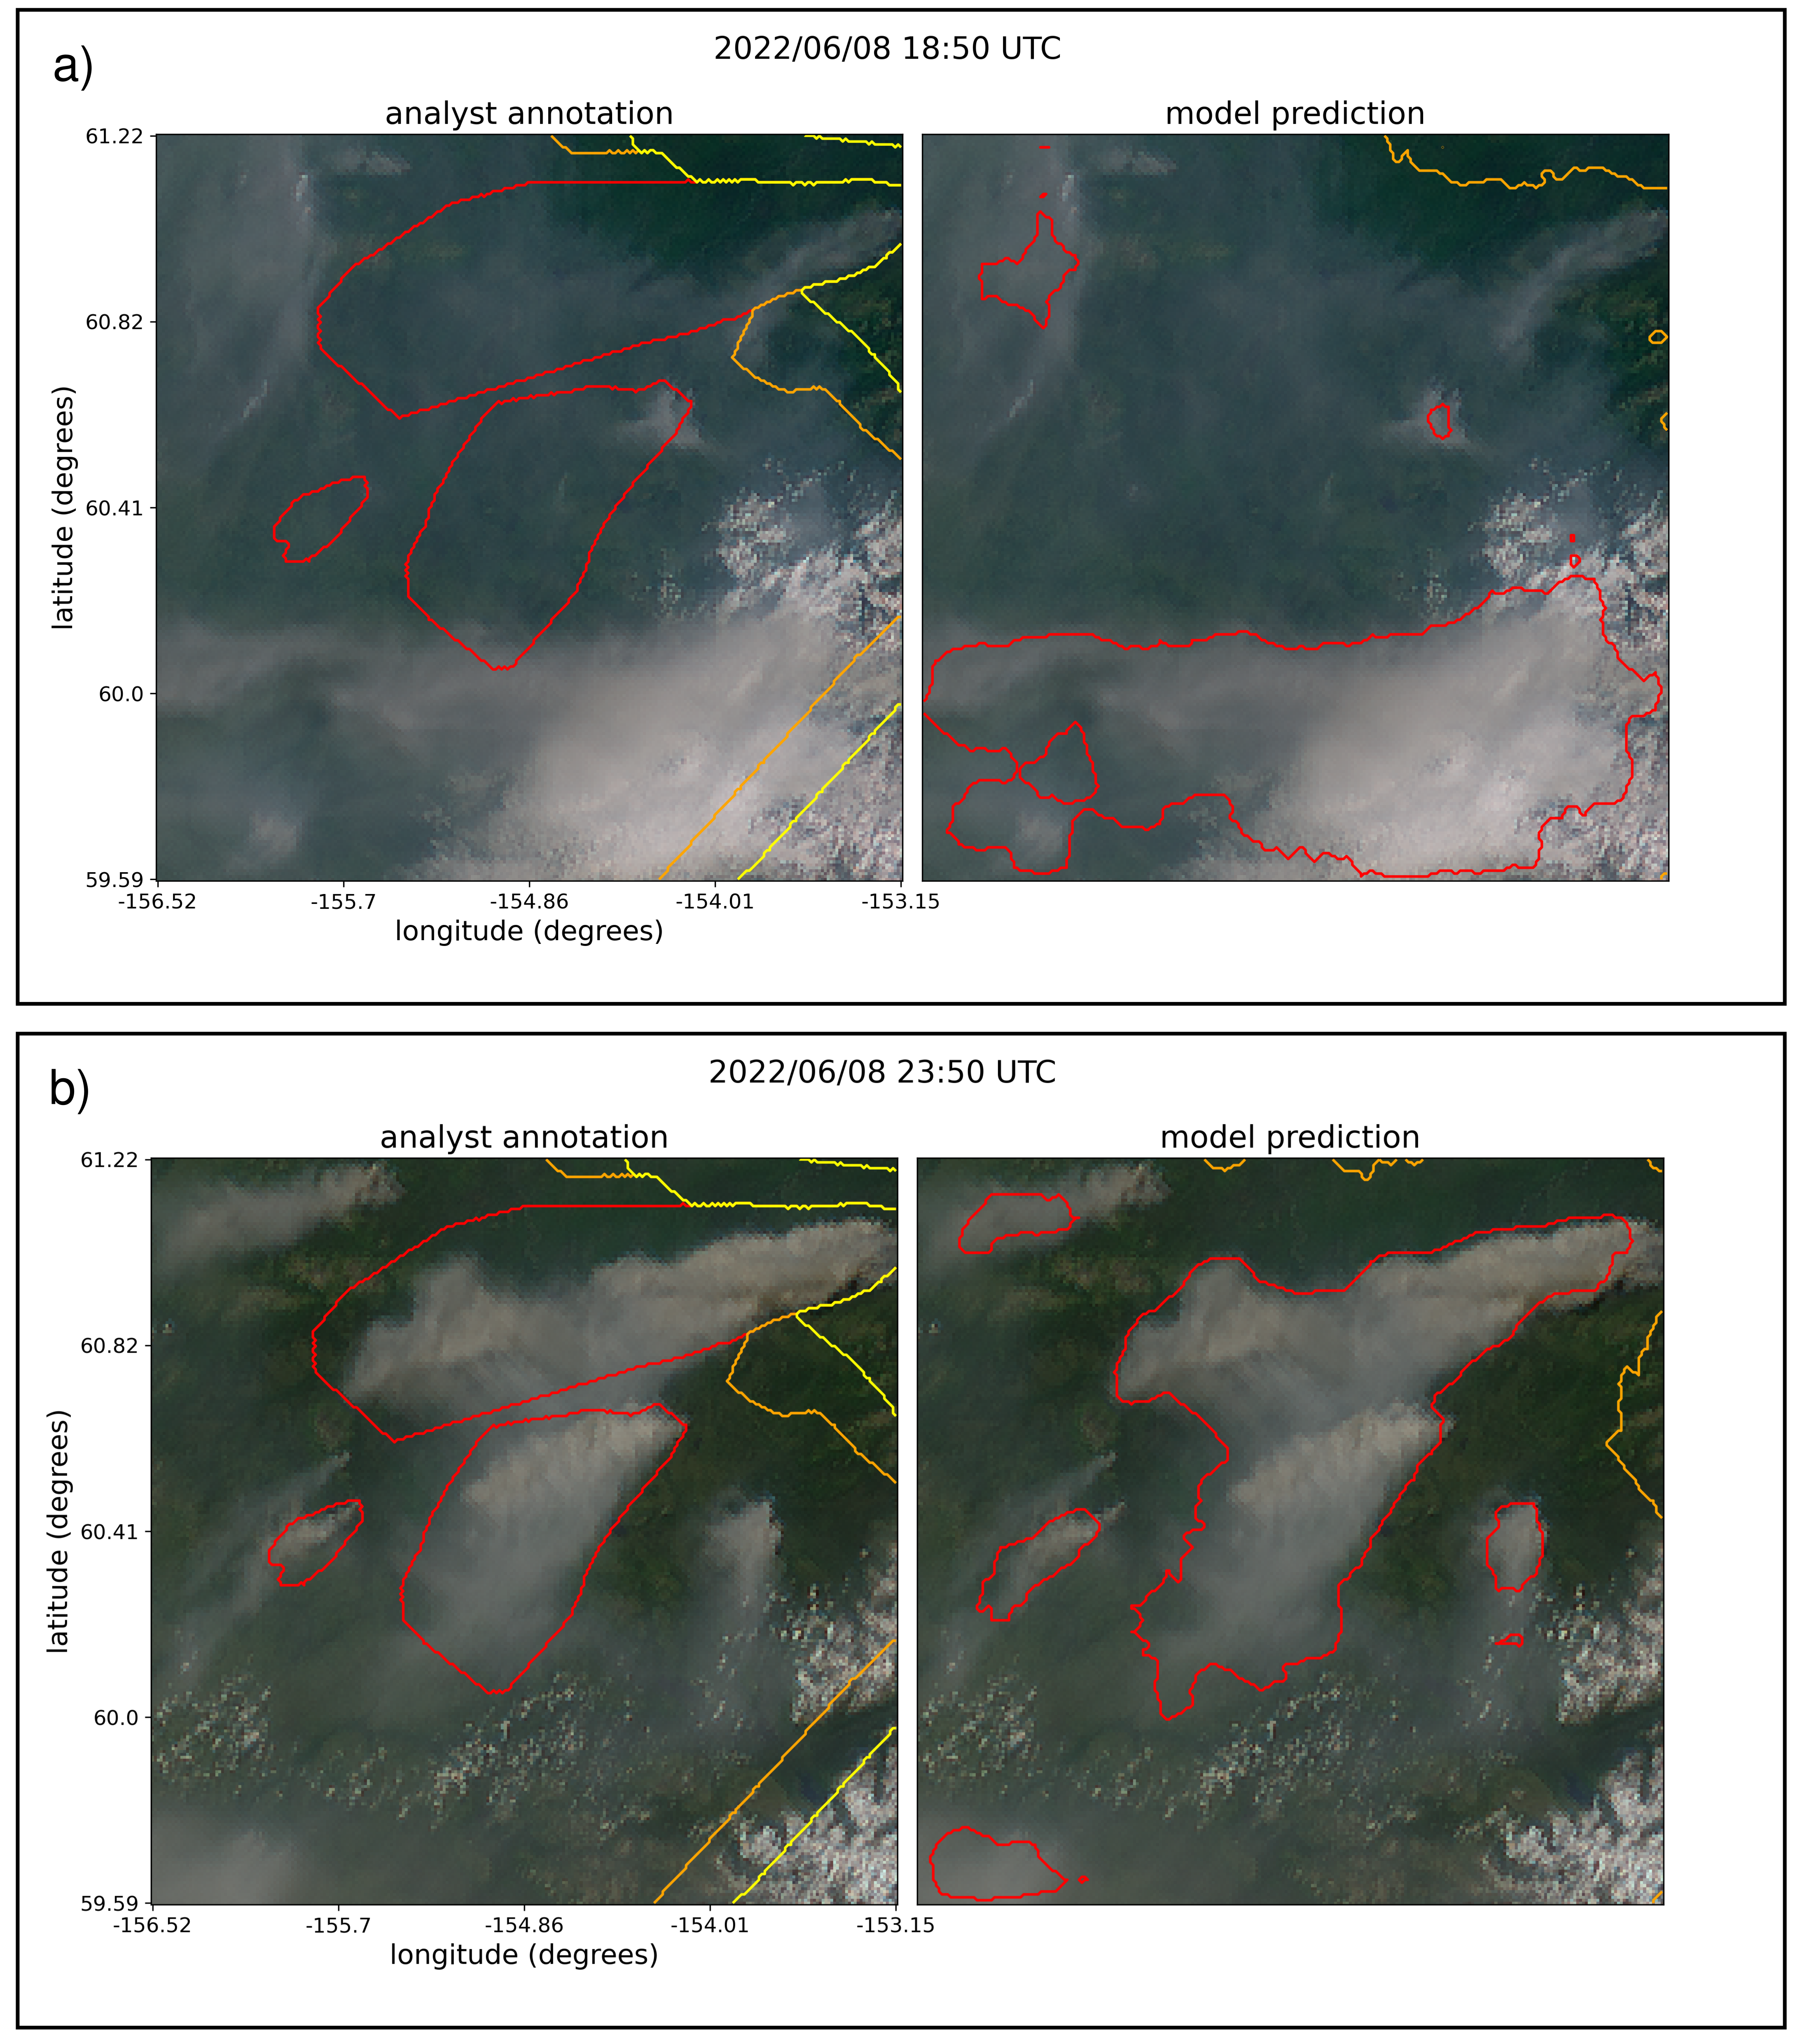
\includegraphics[width=15cm]{figures/ML_better_than_Mei_2.png}
    \caption{GOES-WEST imagery showing smoke on June 8th, 2022 in Alaska where at the coordinates (61°03'N, 156°07'W), daylight was between 12:43-7:53 UTC. The smoke annotations displayed span from 18:50 to 23:50 UTC. a) shows the imagery that was selected using the Mie algorithm, which optimizes for the image closest to sunrise. b) shows the imagery chosen by the pseudo-label that had the highest IoU score. The IoU scores are similar for the low and medium density smoke, but the
    high density smoke IoU for a) is .01 while b) is significantly higher at .59.}\label{ml_vs_mei}
\end{figure}


The result of this study is a curated dataset that can be used to train machine learning models for various wildfire smoke applications. The end goal is to produce a robust and reliable machine learning based approach for detecting wildfires using satellite imagery. That information can be used for wildfire monitoring and as data provided to public health officials for air quality assessments.

%\begin{figure} \label{results}
%    \centering
%    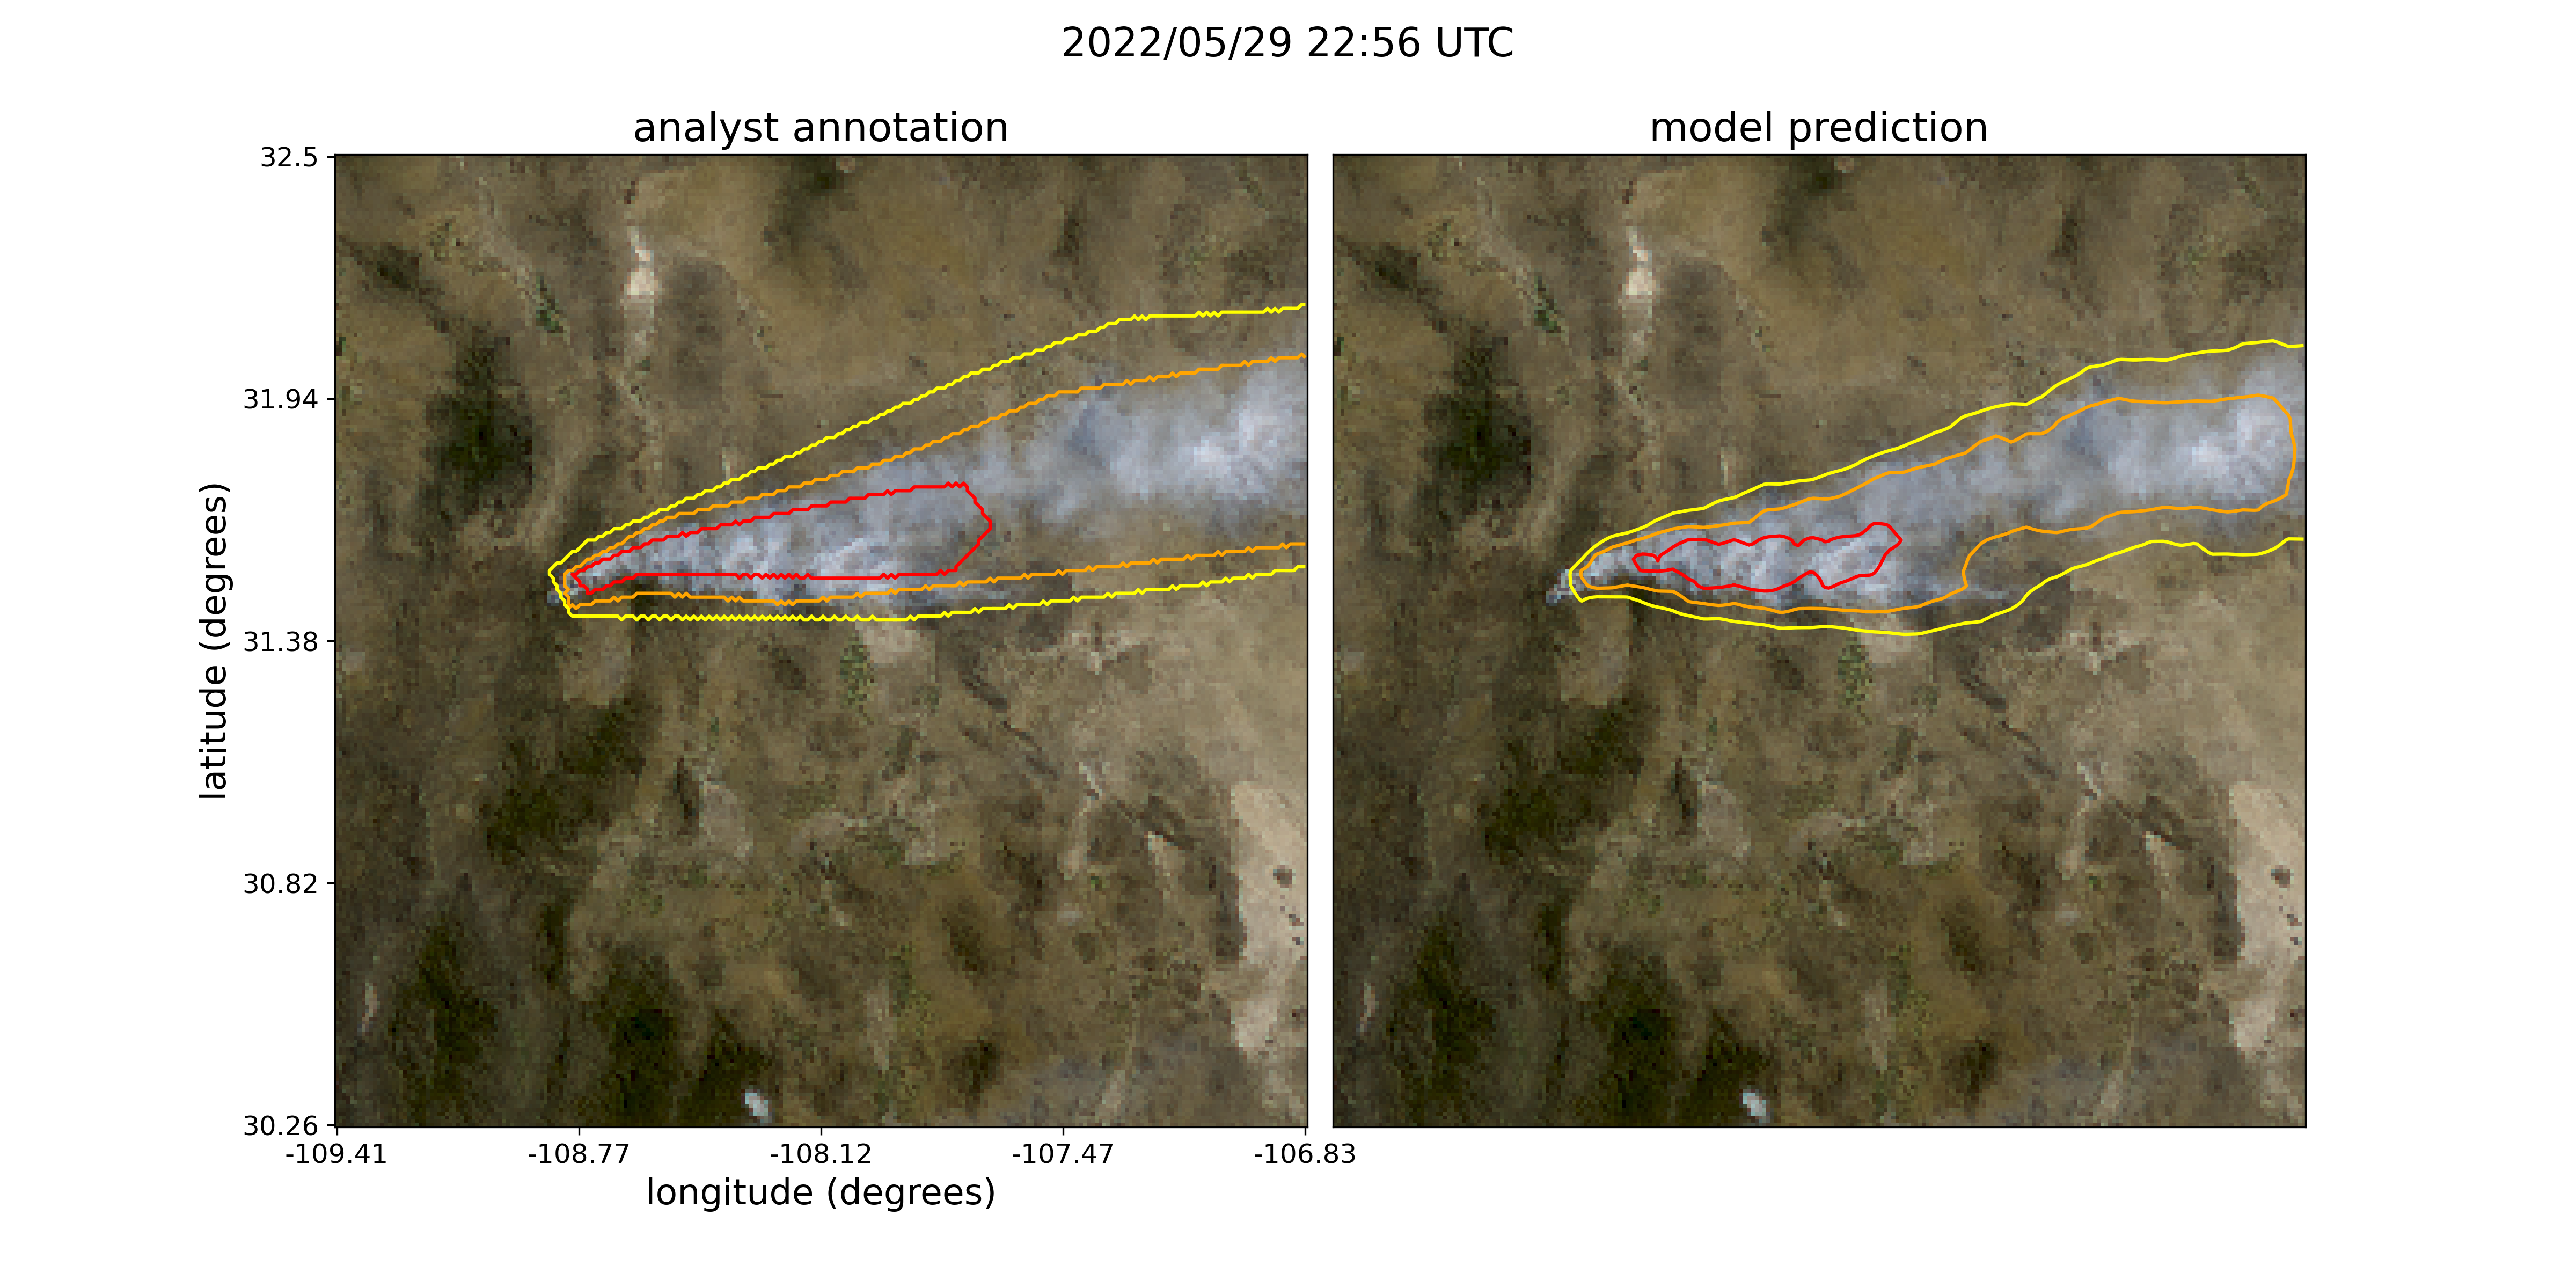
\includegraphics[width=16cm]{figures/results.png}
%    \caption{}
%\end{figure}




\newpage







\bibliography{references}

\end{document}
